\documentclass[parskip=never,landscape,twocolumn]{scrreprt}
\parindent=0pt

\usepackage[ngerman]{babel}
\usepackage{amsmath}

\usepackage{mathptmx}

\usepackage{graphicx}
\usepackage{amsmath}
\usepackage{caption}
\usepackage{xcolor}

\usepackage{multicol}
\usepackage{geometry}
\geometry{a4paper, top=7mm, left=10mm, right=10mm, bottom=5mm, includefoot}

\usepackage{fancybox}

%enumnummerierung ebene2
\renewcommand{\labelenumii}{\arabic{enumii}}

%itemizeabstände
\usepackage{xpatch}
\xpatchcmd{\itemize}
  {\def\makelabel}
  {	\setlength{\itemsep}{0mm}
 	\setlength{\parskip}{0pt}
  	\setlength{\parsep}{0pt}  
  \def\makelabel}
  {}
  {}
  
  \xpatchcmd{\enumerate}
  {\def\makelabel}
  {	\setlength{\itemsep}{0mm}
 	\setlength{\parskip}{0pt}
  	\setlength{\parsep}{0pt}  
  \def\makelabel}
  {}
  {}
  
  \newcommand{\halfpage}[1]{\begin{minipage}{0.49\textwidth} #1 \end{minipage}}

\usepackage{amsfonts}
\usepackage{pdfpages}

\begin{document}
\newcommand{\Naeherung}{\textcolor{purple}{\textbf{Näherung}}}
\definecolor{lgr}{rgb}{0.6,0.6,0.6}
\newcommand{\gray}[1]{\textcolor{lgr}{#1}}

absolute Häufigkeit: $h_i$

relative Häufigkeit: $f_i= \frac{h_i}{n}$

kumulative Häufigkeitsverteilung: H(x) =$\sum_{i:a_i < x} h_i$

empirische Verteilfunktion: $F(x) =  \frac{1}{n} H(x) = \sum_{i:a_i < x} f_i$

arithmetisches Mittel: $\overline{x} = \frac{1}{n} \sum_{i=1}^n x_i = \frac{1}{n} \sum_{i=1}^n h_i a_i $

geometrisches Mittel $\overline{x}_{geom} = \sqrt[n]{\prod_{i=1}^n x_i}$

$\overline{x}_{geom} \leq \overline{x}$

median:  $\tilde{x} = \frac{1}{2} (\lfloor \frac{n}{2} \rfloor + \lceil \frac{n}{2} \rceil )  $ // 50\% größer bzw. kleiner


Modus = häufigster Wert

empirische Varianz: $s^2  = \frac{1}{n-1}\left(\sum_{i=1}^n x_i^2-n\overline{x}^2\right)= \gray{\frac{1}{n-1}\sum_{i=1}^n(x_i-\overline{x})^2}$

Standardabweichung:  $s = \sqrt{varianz} $

Kovarianz: $s_{xy} = \frac{1}{n-1}\sum_{i=1}^n(x_i-\overline{x})(y_i-\overline{y})$

Korrelationskoeffizient: $r_{xy} = \frac{s_{xy}}{s_x\cdot s_y}$

\section*{Bedingte Wahrscheinlichkeiten}

prob(A) = $\frac{\text{|günstige Fälle|}}{\text{| alle Fälle|}}$

$prob(B|A) = \frac{prob(B \cap A)}{prob(A)}$

Unabhängig $\Leftrightarrow prob(A \cap B)=prob(A)\cdot prob(B)$

Satz von Bayes: $prob(B|A) = prob(A|B)\dfrac{prob(B)}{prob(A)}$

$prob(B|A) = \dfrac{prob(A|B)\cdot prob(B)}{prob(B)\cdot prob(A|B) + prob(\overline{B}) \cdot prob(A|\overline{B}) }$


\section*{Erwartungswert}
diskret: $ E(X) = \sum_i^n prob(x_i)\cdot x_i$\\
stetig: $E(X) = \int_{-\infty}^{\infty}xf(x)dx$\\

E(X+Y) = E(X) + E(Y);~~~ E(aX) = aE(X) \\
wenn f symmetrisch um c dann E(X) = c\\
wenn X,Y unabhängig: E(XY) = E(X) $\cdot$ E(Y)

\section*{Kovarianz}
$Cov(X,Y) = E(X \cdot Y) -E(X)E(Y)= \gray{E((X-E(X))\cdot(Y-E(Y)) }$

\section*{varianz}
diskret: $ \sigma^2 = \sum_i^n prob(x_i)\cdot (x_i -E(X))^2$\\
stetig: $ \sigma^2 = \int_{-\infty}^{\infty} (x_i -E(X))^2 f(x) dx$ \\
$\sigma^2 = E(X^2) - E(X)^2$

Var(X+Y) = Var(X) + Var(Y) \gray{ + 2Cov(X,Y)}\\
Var(aX+b) = $a^2$Var(X)


\section*{Standardisierung}
standartisierte Zufallsvariable $Z:=\dfrac{X-\mu}{\sigma}$ => E(X)=0, Var(X)=1


\section*{Verteilunsfunktionen}
Verteilungsfunktion F(x) $= prob(X \leq x)$\\
steigt monoton von 0 nach 1

Dichte: f(x);

$f(x) = F'(x); \\
 F(x) = \int_{-\infty}^xf(t)dt$

\subsection*{Gleichverteilung}
$f(x) = \frac{1}{b-a} falls a < x < b, sonst 0$

$F(x)  = \frac{x-a}{b-a} falls a < x < b, sonst 0 bzw. 1$

E(X) = (b+a)/2

\subsection*{Exponentialverteilung}
$F(x) = 1 - e^{-\lambda x};  \\ f(x) = \lambda e^{-\lambda x}$ für x > 0 \\
E(X) = $1/\lambda$ \gray{= Durchschnittliche Lebensdauer}\\
Var(X) = $1/\lambda^2$
\subsubsection*{\gray{Weibull-Verteilung}}
\gray{$F(x) = 1 - e^{\lambda x^\beta};  \\f(x) = \lambda \beta x^{\beta -1} e^{-\lambda x^\beta}$ für x > 0 }


\subsection*{Hypergeometrische Verteilung}
\Naeherung ei $ 20 n \leq N $  durch Binomialverteilung

N Elemente, M Treffermöglichkeiten, Stichprobe mit n (kein Zurücklegen)

prob(X=x)=$ \dfrac{\left( \! \begin{array}{c}M \\ x \end{array} \! \right) \cdot \left( \begin{array}{c}N-M \\ n-x \end{array}  \right) }{\left( \begin{array}{c}N \\ n \end{array}  \right) }$

$E(X)=n\dfrac{M}{N}~~~
Var(X) = n\dfrac{M}{N} \left( 1- \dfrac{M}{N} \right) \dfrac{N-n}{N-1}
$

\subsection*{binomialverteilung}
Stichprobe mit n, wahrscheinlichkeit pro Teil: p 

$prob(X=x) = \left( \begin{array}{c} n \\ x \end{array} \right) p^x (1-p)^{n-x}$

E(X) = np; ~~~ Var(X) = np(1-p)

\gray{Wenn X = Bi(n;p) und Y = Bi(m;p) unabhängig, dann X + Y = Bi(m+n;p)}

\Naeherung  Bei $n \geq 50, p \leq 0.1 $ durch Poisson-Verteilung mit $\lambda = np$

\Naeherung Bei $np(1-p)\geq 9$: $F_B(x) \approx F_N(x+0.5) = \Phi \left( \dfrac{x+0.5 -np}{\sqrt{np(1-p)}}\right)$


\subsection*{Poisson-Verteilung}
\gray{Auftreten von Ereignis in Zeitinterval:}

$prob(X=x) = \dfrac{\lambda^x}{x!}e^{-\lambda}$

$E(X) = Var(X) = \lambda$

\Naeherung Bei $\lambda \geq 9$ $F_P(x) \approx F_N(x+0.5)=\Phi \left( \dfrac{x+0.5-\lambda}{\sqrt{\lambda}}\right)$


\subsection*{Normalverteilung}
\gray{$f(x) = \frac{1}{\sqrt{2\pi}\sigma} \cdot e^{-0,5\left(\frac{x-\mu}{\sigma}\right)^2}$\\
$\mu = erwartungswert,\sigma^2 = Varianz$\\
$X = N(\mu;\sigma^2), Y = aX + b \Rightarrow Y = N(a\mu + b; a^2\sigma^2)$}

\subsubsection*{Standard-Normalverteilung $z_p$}
\gray{Dichte: $\phi(x) = \frac{1}{\sqrt{2\pi}} \cdot e^{- 0,5 x^2}$\\
Verteilung: $\Phi$ ~~~~~~
$\Phi(-x) = 1-\Phi(x)$\\
E(X) = 0; Var(X) = 1;}


Ablesen an Standard-Normalverteilung: $F(X) = \Phi \left(\dfrac{x-\mu}{\sigma} \right)$, $f(x) = \dfrac{\phi}{\sigma} \left(\dfrac{x-\mu}{\sigma} \right)$

\subsection*{Zentraler Grenzwertsatz, schwache Konvergenz}
Summe über identisch Verteilte Zufallsvariablen $X_i mit E(X_i) = \mu, Var(X_i) = \sigma^2$\\
$X_1 + X_2 + \dots + X_n$\\
Für große n: Normalverteilt mit E = $n\mu$ Var = $n\sigma^2$




\subsection*{Chi-Quadrat (mit m Freiheitsgraden)}
\gray{$ \chi^2(m) = \Sigma_{i=0}^m X_i^2$ für $X_i$ standardnormalverteilt, unabhängig \\
E($\chi^2)$ = m, Var($\chi^2)$ = 2m\\
z.B. $\dfrac{m s^2}{\sigma^2} = \Sigma_{i=1}^{m+1} \left(\dfrac{X_i - \overline{X}}{\sigma}\right)^2$
mit $X_i$ Stichproben aus normalverteilt ist $\chi^2$ verteilt mit m Freiheitsgraden\\
$f_m(x) = \dfrac{x^{m/2-1}}{2^{m/2}\Gamma(m/2)}$ für x>0, sonst 0\\
$\Gamma (x) = \int_0 ^\infty t^{x-1} e^{-1}dt \Leftrightarrow$  x! für $x \in \mathbb{N}$ \\
\Naeherung durch Normalverteilung für m>30: $\chi^2_{m;p} = \sqrt{2m}z_p +m$
}
\subsection*{t-Verteilung  mit m-Freiheitsgraden}
\gray{$t(m) = \dfrac{Z}{\sqrt{X/m}}$ ist t-Verteilt für Z standardnormalverteilt und X Chi-Quadratverteilt\\
E(T) = 0 für m>1, Var(T) = $\dfrac{m}{m-2}$ für m>2\\
z.B. $\dfrac{\overline{X} -\mu }{S/\sqrt{n}}$ für Stichprobe mit Größe n aus Normalverteilter Grundgesamtheit\\
\Naeherung für m>30: $t_{m;p} = \approx \sqrt{\dfrac{m}{m-2}} \Phi(p)$\\
$f_m(x) = \dfrac{\Gamma\left(\dfrac{m+1}{2}\right)}{\sqrt{n\pi}\Gamma( m/2} \left( 1+ \dfrac{x^2}{m}\right)^{-\dfrac{m+1}{2}}$}

\subsection*{F-Verteilung}
\gray{$F(m_1;m_2) = \dfrac{\sqrt{X_1/m_1}}{\sqrt{X_2/m_2}}$ für $X_1 und X_2$ Chi-Quadrat verteilt\\
$E(F) = \dfrac{m_2}{m_2-2}$ für$ m_2 > 2$, $Var(X) = \dfrac{m_2^2(m_1+m_2-2)}{m_1(m_2-4)(m_2-2)^2} $für$ m_2 >4$}

\section*{Zufallsstichproben}
\gray{n gewählte Elemente, die Werte sind zufällig verteilt; wenn ausgreichend Große Grundgesamtheit: Werte unabhängig und gleich verteilt}

\subsection*{Punktschätzer}
\gray{Test einer Verteilung mit zu schätzendem Parameter $\theta$\\
Eigenschaften:\\
\begin{minipage}{0.5\textwidth}
\begin{enumerate}
\item erwartungstreu falls E(T) = $\theta$;~~~~ bias=$E(T)-\theta$
\item asymptotisch erwartungstreu: $\lim_{n\rightarrow \infty} E(T_n) = \theta$
\item konsistent: konvergiert stochastisch gegen $\theta$ \\
( $\lim_{n\rightarrow \infty} prob (|T_n - \theta| <\epsilon ) = 1$ für alle $\epsilon >0 $
\item konsistent im quadratischen Mittel: $\lim_{n\rightarrow \infty} E((T_n-\theta)^2) = 0$\\
bzw. wenn asymptotisch erwartungstreu und Var(X)$\rightarrow$ 0 \\
=> ist auch konsistent; Bsp: arithmetisches Mittel, empirische Verteilung
\end{enumerate}
\end{minipage}
}
\subsubsection*{Maximum-Likelihood}
\gray{asymptotisch erwartungstreu, asymptotisch normalverteilt mit $\mu = \theta$, Varianz minimal}

\begin{minipage}{0.25\textwidth}
\begin{enumerate}
\item Berechne f(x) wenn nicht gegeben \\(Ableiten von F(x) nach x)
\item $L = \prod_{i=1}^n f(x_i,\theta)$
\item berechne log(L) 
\item berechne maximum von L \\\textbf{(ABLEITEN, = 0 } 
\end{enumerate}
\end{minipage}
\begin{minipage}{0.25\textwidth}
\textcolor{gray}{
\begin{enumerate}
\item Bsp: f(x) = $\lambda e^ {-\lambda x_i}$\\
\item $ L = \prod_{i=1}^n \lambda e^ {-\lambda x_i}$
\item $	z.B. log(L) = n ln(\lambda) -\lambda \sum_{i=1}^n x_i $
\item $n/\lambda - \sum_{i=1}^n x_i \dots$ \textbf{=0}\\
auflösen $\lambda = n/ \sum_{i=1}^n x_i$
\end{enumerate}}
\end{minipage}

\newcommand{\bc}{\textcolor{orange}{c}}
\newcommand{\red}[1]{\textcolor{red}{#1}}

Logarithmen:
\begin{itemize}
\item $log(\red{xy}) = log(\red{x}) + log(\red{y})$
\item $log(x^{\bc}) = \bc log(x)$
\item $e^{log(x)} = x$
\end{itemize}

\subsubsection*{Least Squares/Regressionsrechnung (Gauß):}
Zu nähernde Funktion f(x) in Parameterform, z.B. Gerade: y= mx+t\\
Stichprobe mit Wertepaaren: $(x_1,y_1)\dots (x_n,y_n)$

\begin{enumerate}
\item Bilde s$\Delta : = \sum_{i=1}^n(y_i - f(x_i))^2$
\item Leite nach jedem Parameter ab, setze gleich Null, bestimme Parameter
\end{enumerate}

Alternative für Geraden: $m= r_xy\frac{x_y}{s_x}, d = \overline{y}-k\overline{x}$

\subsection*{Intervallschätzung}
Irrtumswahrscheinlichkeit: $\alpha$ 
Konfidenzniveau: $1-\alpha$\\

zweiseitiges Konfidenzintervall: Intervall zwischen $\overline{x} \pm Abweichung$ ~~~~ //siehe Folgende
einseitiges Konfidenzintervall: $[-\infty; \overline{x} + Abweichung]$

\textbf{wenn $\sigma$ nicht gegeben }\\
Abweichung(zweiseitig): $\dfrac{s}{\sqrt{n}} \cdot t_{n-1;~ 1-\alpha/2}$\\
Abweichung(einseitig): $\dfrac{s}{\sqrt{n}} \cdot t_{n-1;~ 1-\alpha}$

\textbf{wenn $\sigma$ gegeben}\\
Abweichung(zweiseitig): $\dfrac{\sigma}{\sqrt{n}}\cdot  z_{1-\alpha/2}$\\
Abweichung(einseitig): $\dfrac{\sigma}{\sqrt{n}} \cdot z_{1-\alpha}$


\section*{t-Test}
Stichprobe mit Mittelwert $\overline{x}$; Hypothese $H_0: \mu = \mu_0$\\
Prüfwert: $z= \dfrac{\overline{x} - \mu_0}{s/\sqrt{n}}$

\subsection*{zweiseitig}
Ablehnungsbereich: $|z| > t_{n-1;1-\alpha/2} => H_0 $muss verworfen werden 
\subsection*{einseitig}
Ablehnungsbereich: $|z| > t_{n-1;1-\alpha} => H_0 $muss verworfen werden 


\section*{Chi-Quadrat-Anpassungstest}
Test auf Verteilung = vermutete Verteilung\\
Vorraussetzung: große Stichprobe: ($np_i \geq 5$) für alle i

\begin{enumerate}
\item Teile Werte in Intervalle $I_i$ auf; \gray{// Aus angabe entnehmen}
\item $h_i:$ Anzahl der Werte in $I_i$ \gray{// Aus angabe entnehmen} 
\item $p_i$ : Wahrscheinlichkeit von $I_i$ laut vermuteter Verteilung \gray{// Berechne aus Verteilungsfunktion \textcolor{lightgray}{obere Grenze -untere Grenze}}\\

\item $y = \gray{ \sum_{i=1}^k \dfrac{(h_i -np_i)^2}{n p_i} }= 1/n \left( \sum_{i_1}^k \dfrac{h_i^2}{p_i} \right) -n $
\gray{ist asymptotisch  $\chi^2 (k-1)$ verteilt }\\

\item 0 geschätzte Parameter: Ablehnungsbereich: y > $\chi^2_{k-1;1-\alpha}$

g geschätzte Parameter: Ablehnungsbereich: y > $\chi^2_{k-1-g;1-\alpha}$

\end{enumerate}

\section*{Ableitungen}
Kettenregel: $f(g)' = f'(g) \cdot g'$ // Nachleiten 

Bsp: $(e^{-5x^2})' = e^{-5x^2} \cdot (-10x)$

Bsp: $((x-4)^2 +(4x+5)^2)' = 2(x-4) + 2(4x+5)\cdot4 $

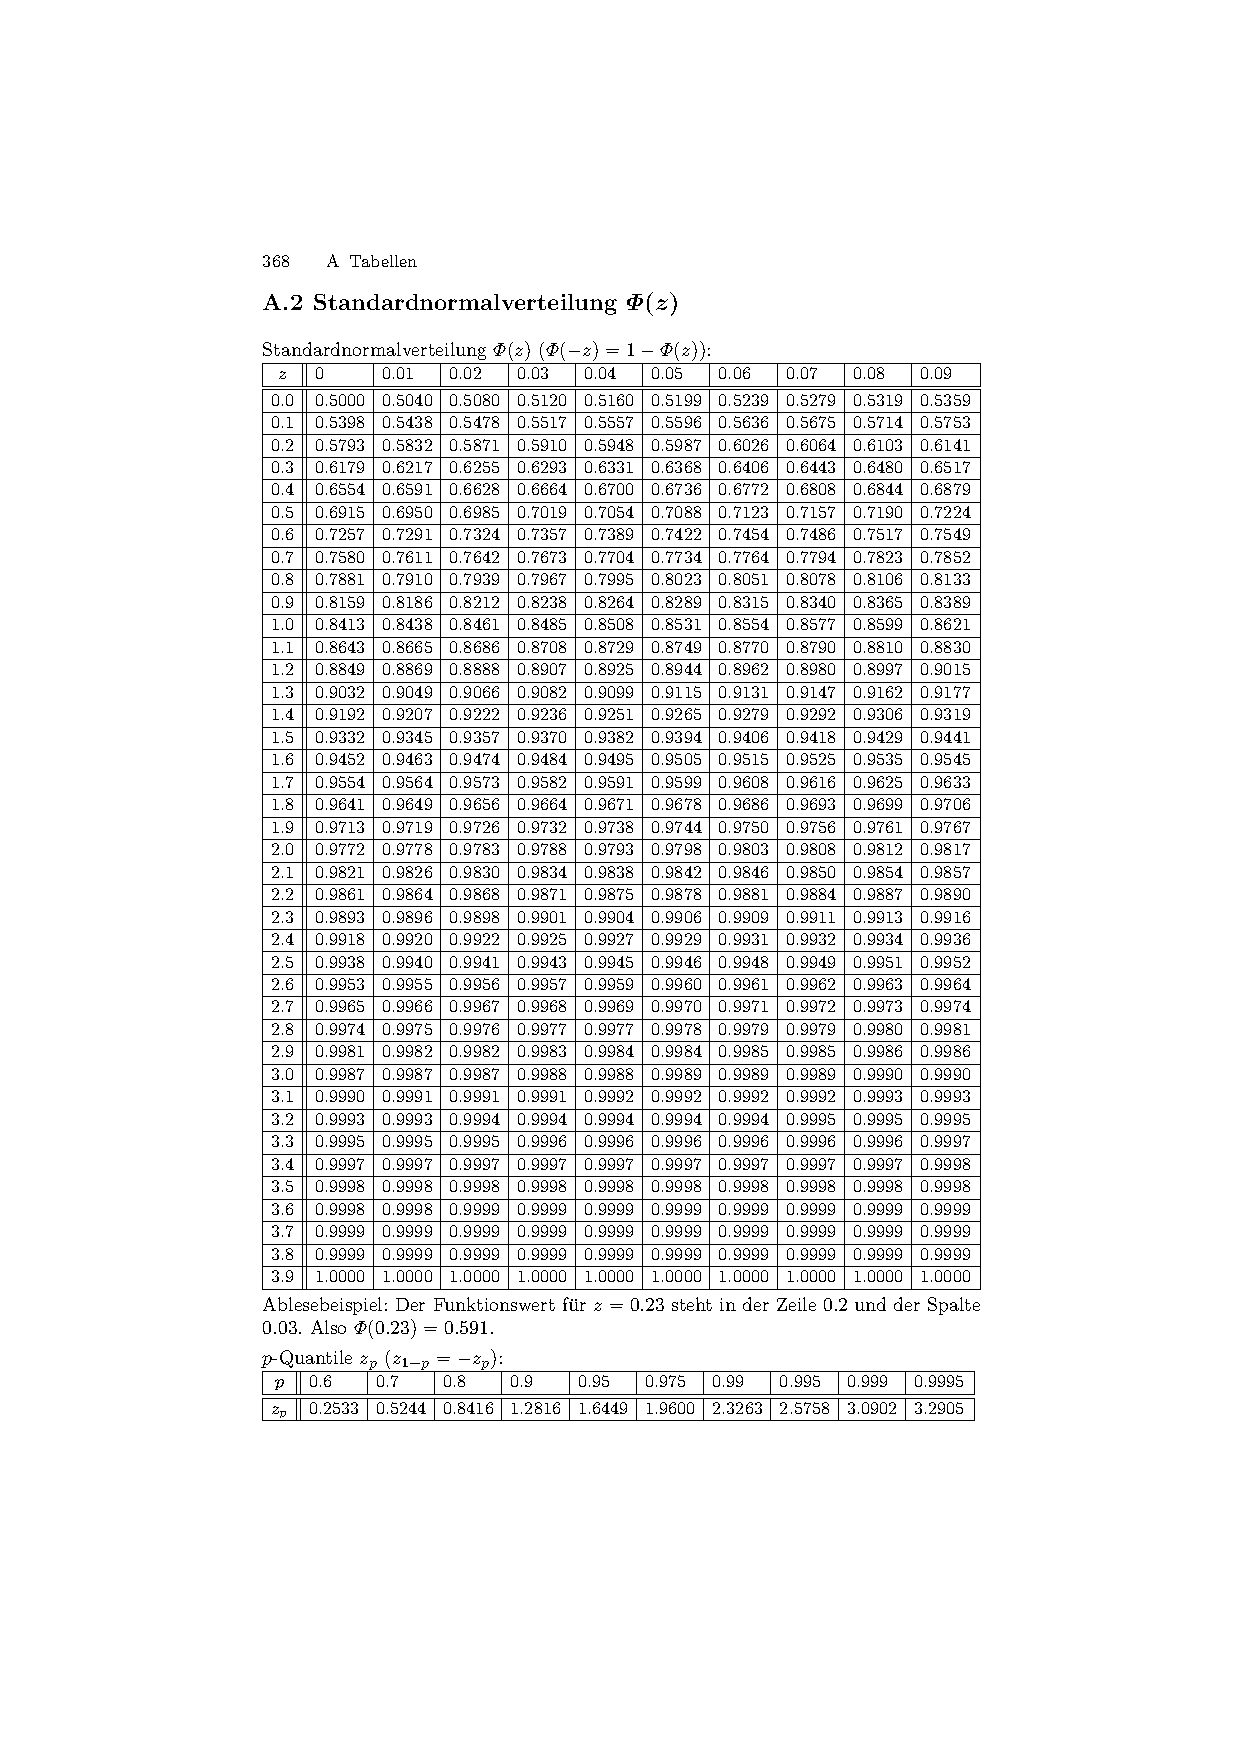
\includepdf[pages={1},nup=2x1,openright=true]{TT2.pdf}
\includepdf[pages={2-},nup=2x1]{TT2.pdf}

\end{document}